% 图 2.2 —— 手工重建（三个自由曲线团块 A/B/C + 两条映射箭头 f、g + 三个圆点）
%
% 曲线全部是**显式三次贝塞尔**：团块 = 周期三次 B 样条最小二乘拟合（C² 闭合），
% 箭头 = 开曲线 B 样条拟合。控制点由 `bezfit.py` 出，逐段偏差可量化。
%   · 团块轮廓  内部空白区的边界 → 法向吸附到笔画中轴 → 稳健拟合（IRLS 降权离群点）
%   · 箭头轴心  按列取质心**实测**，不是照描摹点发的（见 checks/gen22.py 的注释）
%   · 线宽      团块/箭头实测 5.0
\documentclass[12pt]{standalone}
\usepackage{fontspec}
\setsansfont{Arial}
\usepackage{tikz}

\begin{document}
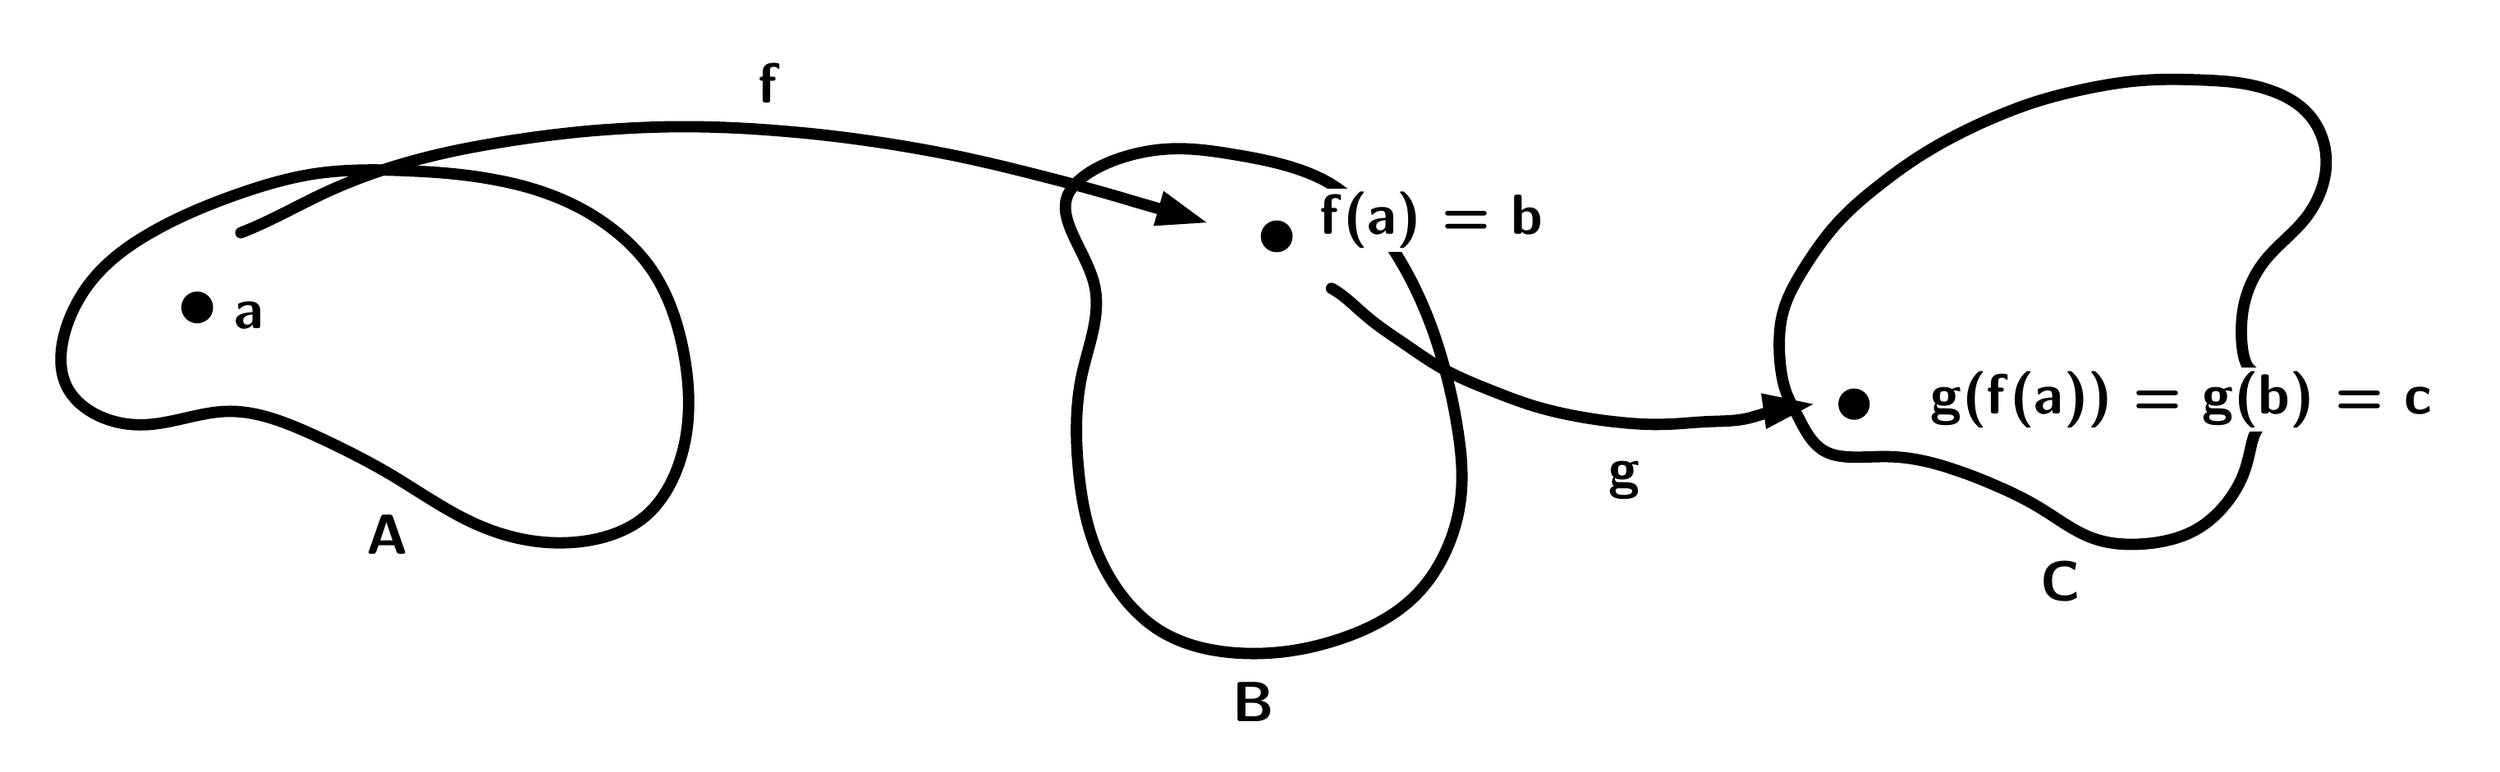
\begin{tikzpicture}[x=1pt, y=-1pt, line width=5.0pt, line cap=round, line join=round]

  % ════ 三个团块 ════
  %% 团块 A：18 控制点 / 18 段三次贝塞尔（周期 C² 闭合）
  \draw[line width=5.0pt, line cap=round, line join=round]
      (89.4,77.4)
    .. controls (76.8,82.1) and (64.7,87.4) .. (53.5,94.2)
    .. controls (42.4,100.9) and (32.2,109.2) .. (25.2,121.0)
    .. controls (18.1,132.9) and (14.1,148.2) .. (18.9,159.2)
    .. controls (23.7,170.2) and (37.2,176.8) .. (50.6,177.1)
    .. controls (63.9,177.5) and (77.0,171.5) .. (89.9,171.2)
    .. controls (102.9,170.8) and (115.7,176.0) .. (127.9,181.5)
    .. controls (140.1,187.1) and (151.7,192.9) .. (163.1,199.7)
    .. controls (174.5,206.6) and (185.7,214.4) .. (197.6,220.0)
    .. controls (209.6,225.6) and (222.3,229.0) .. (235.7,229.1)
    .. controls (249.2,229.2) and (263.4,226.0) .. (273.4,217.9)
    .. controls (283.4,209.7) and (289.2,196.6) .. (291.7,183.3)
    .. controls (294.1,170.1) and (293.2,156.8) .. (290.6,143.8)
    .. controls (288.0,130.9) and (283.6,118.3) .. (276.0,107.6)
    .. controls (268.3,96.9) and (257.3,88.1) .. (245.6,81.8)
    .. controls (233.9,75.6) and (221.5,71.7) .. (208.5,69.3)
    .. controls (195.6,66.8) and (182.1,65.7) .. (168.6,65.2)
    .. controls (155.0,64.6) and (141.4,64.6) .. (128.1,66.6)
    .. controls (114.8,68.7) and (101.9,72.8) .. (89.4,77.4)
    -- cycle;
  %% 团块 B：16 控制点 / 16 段三次贝塞尔（周期 C² 闭合）
  \draw[line width=5.0pt, line cap=round, line join=round]
      (471.7,115.6)
    .. controls (474.7,128.9) and (469.0,142.0) .. (466.1,155.4)
    .. controls (463.3,168.8) and (463.3,182.5) .. (464.6,196.0)
    .. controls (465.8,209.4) and (468.2,222.7) .. (473.8,235.3)
    .. controls (479.4,247.9) and (488.2,259.8) .. (499.6,267.2)
    .. controls (511.0,274.6) and (525.0,277.4) .. (538.5,277.8)
    .. controls (551.9,278.2) and (564.8,276.2) .. (577.7,272.1)
    .. controls (590.7,268.0) and (603.6,261.8) .. (613.2,252.1)
    .. controls (622.8,242.4) and (629.1,229.1) .. (631.8,216.2)
    .. controls (634.5,203.4) and (633.5,190.9) .. (631.3,177.7)
    .. controls (629.2,164.4) and (625.7,150.3) .. (621.1,136.9)
    .. controls (616.4,123.6) and (610.5,111.1) .. (602.9,99.4)
    .. controls (595.4,87.8) and (586.3,77.1) .. (574.3,70.2)
    .. controls (562.2,63.4) and (547.2,60.4) .. (533.5,58.1)
    .. controls (519.7,55.8) and (507.2,54.1) .. (492.7,57.1)
    .. controls (478.1,60.0) and (461.6,67.7) .. (459.2,78.2)
    .. controls (456.8,88.8) and (468.6,102.2) .. (471.7,115.6)
    -- cycle;
  %% 团块 C：31 控制点 / 31 段三次贝塞尔（周期 C² 闭合）
  \draw[line width=5.0pt, line cap=round, line join=round]
      (933.2,25.4)
    .. controls (924.9,26.0) and (916.9,27.3) .. (908.7,29.0)
    .. controls (900.5,30.7) and (892.2,32.8) .. (884.2,35.4)
    .. controls (876.2,38.1) and (868.4,41.3) .. (860.7,44.8)
    .. controls (853.0,48.4) and (845.4,52.3) .. (838.1,56.8)
    .. controls (830.8,61.2) and (823.8,66.3) .. (817.2,71.5)
    .. controls (810.5,76.7) and (804.2,82.1) .. (798.5,88.4)
    .. controls (792.8,94.7) and (787.8,102.0) .. (783.4,109.1)
    .. controls (779.0,116.3) and (775.2,123.2) .. (773.8,131.9)
    .. controls (772.4,140.6) and (773.2,151.1) .. (774.7,157.9)
    .. controls (776.3,164.7) and (778.4,167.9) .. (781.2,173.2)
    .. controls (784.0,178.6) and (787.4,186.1) .. (794.0,189.2)
    .. controls (800.7,192.4) and (810.6,191.1) .. (819.3,191.1)
    .. controls (828.0,191.1) and (835.5,192.5) .. (843.4,194.7)
    .. controls (851.3,197.0) and (859.7,200.1) .. (867.5,203.5)
    .. controls (875.3,206.8) and (882.5,210.3) .. (889.6,214.8)
    .. controls (896.7,219.2) and (903.8,224.6) .. (911.8,227.3)
    .. controls (919.9,230.1) and (928.9,230.2) .. (937.3,229.2)
    .. controls (945.7,228.1) and (953.5,225.8) .. (960.4,220.8)
    .. controls (967.3,215.8) and (973.2,208.3) .. (976.5,200.9)
    .. controls (979.8,193.5) and (980.4,186.4) .. (981.9,182.3)
    .. controls (983.3,178.3) and (985.6,177.3) .. (986.1,172.9)
    .. controls (986.5,168.4) and (985.2,160.4) .. (983.4,156.6)
    .. controls (981.6,152.8) and (979.4,153.2) .. (978.0,148.6)
    .. controls (976.5,144.1) and (975.8,134.6) .. (977.3,126.0)
    .. controls (978.8,117.5) and (982.5,109.9) .. (987.8,103.6)
    .. controls (993.1,97.3) and (1000.1,92.2) .. (1005.2,85.5)
    .. controls (1010.3,78.7) and (1013.7,70.3) .. (1013.8,61.9)
    .. controls (1014.0,53.6) and (1011.0,45.3) .. (1005.2,39.4)
    .. controls (999.5,33.4) and (991.0,29.9) .. (982.7,27.9)
    .. controls (974.4,25.9) and (966.2,25.5) .. (958.0,25.2)
    .. controls (949.7,24.9) and (941.4,24.8) .. (933.2,25.4)
    -- cycle;

  % ════ 箭头 f：A 内 → 越过 B 顶 → 指向 b 点 ════
  \draw[line width=5.0pt, line cap=round, line join=round]
      (96.0,92.5)
    .. controls (108.7,87.6) and (120.4,80.8) .. (132.6,75.1)
    .. controls (144.8,69.4) and (157.6,64.8) .. (170.6,61.2)
    .. controls (183.6,57.5) and (196.9,54.9) .. (210.2,52.7)
    .. controls (223.6,50.5) and (237.0,48.8) .. (250.4,47.6)
    .. controls (263.9,46.5) and (277.4,45.8) .. (290.9,45.8)
    .. controls (304.4,45.8) and (317.9,46.4) .. (331.4,47.5)
    .. controls (344.8,48.5) and (358.3,50.0) .. (371.6,51.9)
    .. controls (385.0,53.8) and (398.3,56.1) .. (411.5,58.8)
    .. controls (424.8,61.6) and (437.9,64.8) .. (451.0,68.2)
    .. controls (464.0,71.5) and (477.1,75.1) .. (490.0,79.0);
  % 箭杆接进三角（补缝，见 arrow_tail 注释）
  \draw (490.0,79.0) -- (506.9,83.9);
  \fill (521.0,88.0) -- (497.7,89.5) -- (502.1,74.1) -- cycle;

  % ════ 箭头 g：B 内 → 指向 c 点 ════
  \draw[line width=5.0pt, line cap=round, line join=round]
      (576.0,117.0)
    .. controls (581.8,120.1) and (586.6,125.3) .. (591.8,129.6)
    .. controls (597.0,134.0) and (602.5,137.6) .. (608.1,141.4)
    .. controls (613.6,145.2) and (619.1,149.1) .. (625.0,152.4)
    .. controls (630.9,155.7) and (637.1,158.3) .. (643.3,160.8)
    .. controls (649.6,163.3) and (655.8,165.8) .. (662.2,167.9)
    .. controls (668.6,170.0) and (675.1,171.6) .. (681.7,172.9)
    .. controls (688.3,174.2) and (695.0,175.2) .. (701.7,175.9)
    .. controls (708.4,176.6) and (715.1,177.1) .. (721.8,176.9)
    .. controls (728.5,176.8) and (735.3,176.0) .. (742.0,175.7)
    .. controls (748.7,175.4) and (755.3,175.6) .. (762.0,173.5);
  % 箭杆接进三角（补缝，见 arrow_tail 注释）
  \draw (762.0,173.5) -- (773.5,170.1);
  \fill (788.0,168.0) -- (767.3,179.0) -- (765.1,163.2) -- cycle;

  % ════ 三个实心圆点 ════
  \fill (551.9,94.1) circle (7.0);
  \fill (806.0,168.0) circle (6.9);
  \fill (76.8,125.4) circle (7.0);

  % ════ 标签 ════
  \node[anchor=center,inner sep=1.5pt,fill=white,font=\fontsize{33.0}{41.2}\selectfont] at (99.6,129.1) {\textsf{\textbf{\textit{a}}}};
  \node[anchor=center,inner sep=1.5pt,fill=white,font=\fontsize{28.8}{36.0}\selectfont] at (160.6,225.5) {\textsf{\textbf{\textit{A}}}};
  \node[anchor=center,inner sep=1.5pt,fill=white,font=\fontsize{31.0}{38.8}\selectfont] at (541.8,299.0) {\textsf{\textbf{\textit{B}}}};
  \node[anchor=center,inner sep=1.5pt,fill=white,font=\fontsize{29.0}{36.2}\selectfont] at (897.0,246.0) {\textsf{\textbf{\textit{C}}}};
  \node[anchor=center,inner sep=1.5pt,fill=white,font=\fontsize{34.1}{42.6}\selectfont] at (329.0,26.6) {\textsf{\textbf{\textit{f}}}};
  \node[anchor=center,inner sep=1.5pt,fill=white,font=\fontsize{34.8}{43.5}\selectfont] at (705.0,201.4) {\textsf{\textbf{\textit{g}}}};

  % ════ 说明文字 ════
  \node[anchor=center,inner sep=1.5pt,fill=white,font=\fontsize{29.1}{36.4}\selectfont] at (620.0,87.0) {\textsf{\textbf{\textit{f}(\textit{a}) = \textit{b}}}};
  \node[anchor=center,inner sep=1.5pt,fill=white,font=\fontsize{31.1}{38.9}\selectfont] at (950.0,166.0) {\textsf{\textbf{\textit{g}(\textit{f}(\textit{a})) = \textit{g}(\textit{b}) = \textit{c}}}};

  \path[use as bounding box] (0,0) rectangle (1080,320);
\end{tikzpicture}
\end{document}
